\subsubsection{Consideraciones de diseño}
Se diseñó una fuente de tensión regulada con limitación de corriente enfocados en alcanzar la menor disipación de potencia posible, utilizando la mínima cantidad de componentes necesaria para su funcionamiento. Los requerimientos de la misma son los siguientes:

\textbf{Corriente de salida:}
\begin{equation}
	I = [0\ mA, 200\ mA]
\end{equation}

\textbf{Tensión de salida:}
\begin{equation}
V_{o} = 5 \pm 3\%
\end{equation}

Dado que se busca minimizar la cantidad de componentes utilizados, se decidió utilizar una protección del tipo lineal en vez de foldback.

A continuación se explica brevemente el primer diseño propuesto para luego dar lugar a una explicación más detallada sobre un versión optimizada de la fuente.

\subsubsection{Primer diseño propuesto}
El primer diseño que se propuso fue el siguiente:
\begin{figure}[H]
	\centering
	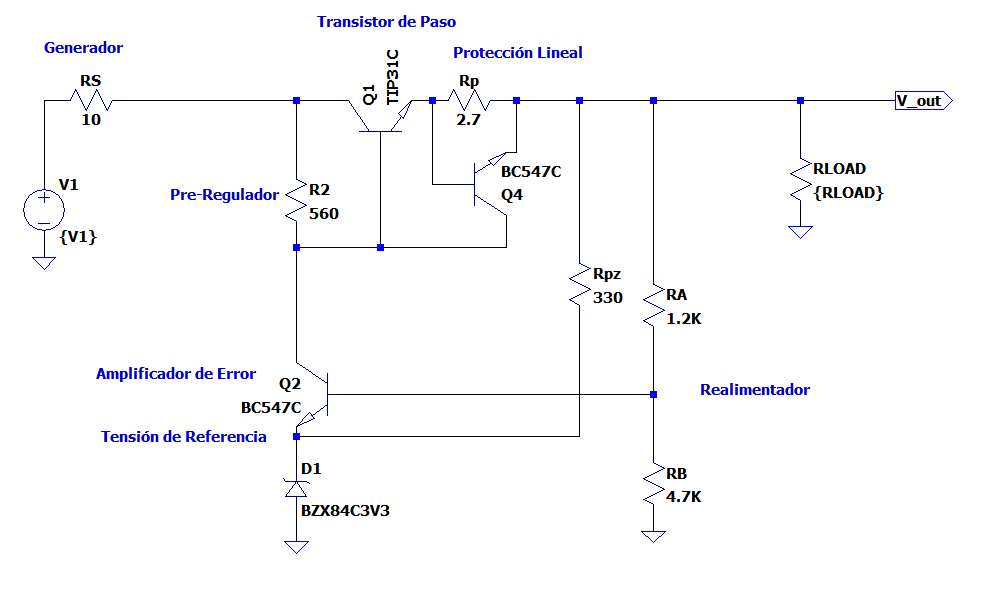
\includegraphics[width=0.7\linewidth]{ImagenesEjercicio1/ImagenCircuitoFV}
	\caption{Fuente de tensión regulada con limitación de corriente}
	\label{fig:imagencircuito}
\end{figure}

La \textbf{tensión de referencia} le permite al amplificador de error saber cuando debe compensar su salida ante variaciones en la tensión de salida. 
En este caso se decidió que la tensión de referencia fuese de $V_{ref} = 4\ V$ dado que era posible utilizar una combinación de valores comerciales de resistencias tal que:
\begin{equation}
	V_{ref}  = V_{o} \cdot \frac{R_B}{R_A + R_B}
\end{equation} 
Dado que 
\begin{equation}
	V_{ref} \approx 5 \cdot 0.7966
\end{equation}
\begin{equation}
	V{ref} = 4 \pm 0.5 \%
\end{equation}

Para diseñar el Pre-Regulador se tuvo en cuenta la ganancia de corriente del transistor de paso \textbf{Q1}.
\begin{figure}[H]
	\centering
	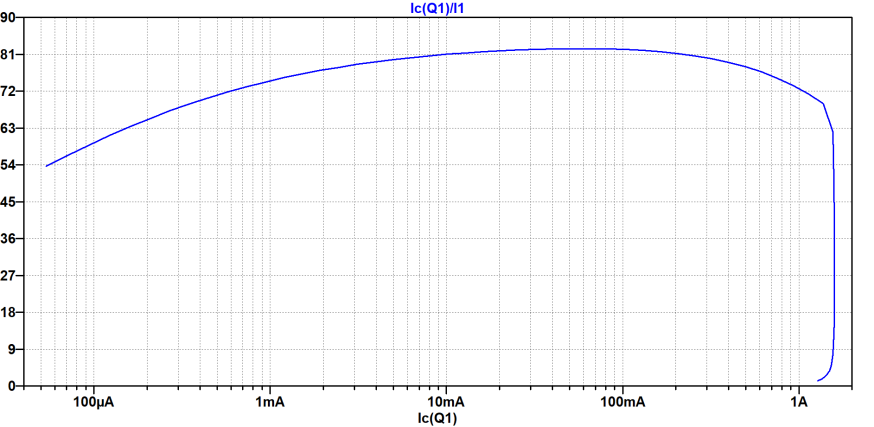
\includegraphics[width=0.7\linewidth]{ImagenesEjercicio1/BetaTPasoFV}
	\caption{Curva de la ganancia de corriente $\beta$. $V_{ce}=2.52$}
	\label{fig:betatpasofv}
\end{figure}

Cuando la carga es mínima, el transistor de paso experimenta el mayor flujo de corriente. En este caso ese valor es de unos $205\ mA$ aproximadamente. Volviendo a la Figura (\ref{fig:betatpasofv}), se ves que la ganancia de corriente se ubica por encima de $80$. 
Por lo tanto podemos obtener la siguiente expresión para el calculo de $R_2$. Debemos tener en cuenta que esto ocurre cuando el transistor \textbf{Q2} se encuentra en corte.

\begin{equation}
R_{2} = \frac{V_{gen}-R_{g}\cdot I_{o_{max}} - (V_o + V_{be_{Q3}} + V_{be_{Q1}}  )}{I_o} \cdot \beta
\end{equation}
\begin{equation}
R_{2} = \frac{10 - 10 \Omega \cdot 205mA - (5V + 0.580 +0.7)  }{200mA} \cdot 80
\end{equation}
\begin{equation}
R_{2} = 652 \Omega
\end{equation}

El valor de resistencia obtenido es un valor \textbf{no} comercial. Se podría ir por el valor más próximo, $680 \ \Omega$ pero este valor no cumple con las especificaciones. Por lo tanto se opta por el valor comercial menor más próximo, es decir $560 \ \Omega$.

\subsubsection{Circuito de Protección}
La resistencia de protección se calculo teniendo en cuenta que la corriente de emisor del transistor de paso incluía la corriente necesaria para la polarización del diodo Zener. 
\begin{equation}
	R_p = \frac{V_{be_{Q3}}}{I_{emisor}}
\end{equation}

El \textbf{elemento de referencia} en este caso se escogió como la combinación de la tensión de Zener y $V_{be_{ON}}$
\begin{equation}
	V_{ref} = V_{zener} + V_{be_{ON}}
\end{equation}

Para poder obtener la característica de salida, se puede optar por usar la directiva de spice \textit{.step param}, o bien simular una carga variable mediante el uso de una fuente de corriente. El ultimo método ofrece una mayor velocidad de simulación y gráficos de mayor calidad.

\begin{figure}[H]
	\centering
	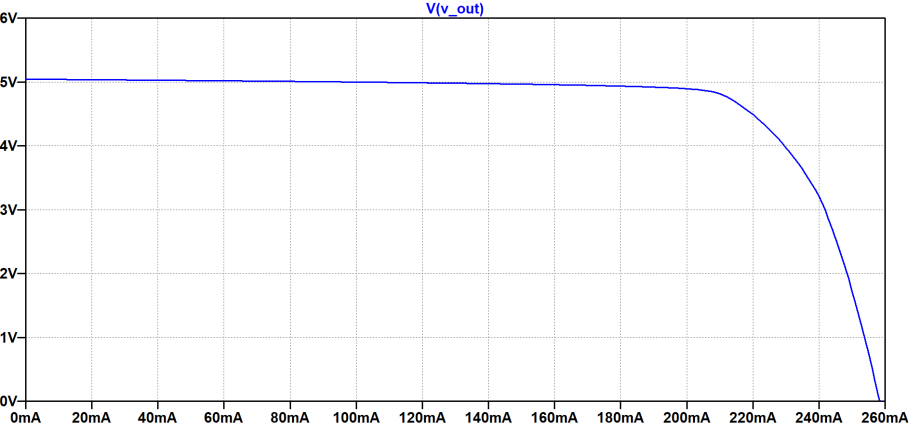
\includegraphics[width=0.7\linewidth]{ImagenesEjercicio1/CaracteristicaDeSalidaConGrillaFV}
	\caption{Característica de Salida Diseño 1}
	\label{fig:caracteristicadesalidacongrillafv}
\end{figure}

Este gráfico indica que el circuito ofrece una buena regulación de tensión dentro del rango de corriente requerido. Sin embargo se nota algo inesperado, a partir de los $200 \ mA$ no hay una caída abrupta de la tensión, sino más bien una caída suave hacia 0. Se estudia esto en más detalle en la próxima sección.

\subsection{Segunda iteración de diseño}
Utilizar la menor cantidad de componentes ofrece varios beneficios como por ejemplo, menos efectos de las tolerancias, mayor aprovechamiento del espacio y mayor sencillez de diseño. A continuación se presenta el diseño resultante:
\begin{figure}[H]
	\centering
	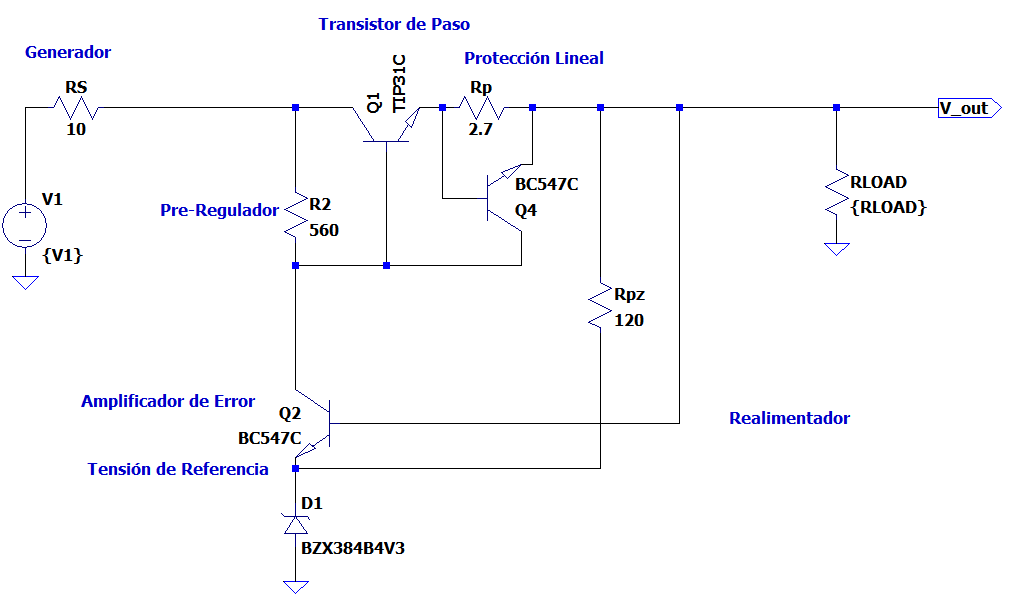
\includegraphics[width=0.7\linewidth]{ImagenesEjercicio1/ImagenCircuitoFLcasiPelada.PNG}
	\caption{Fuente de tensión regulada con optimización}
	\label{fig:imagencircuitofl}
\end{figure}

En esta oportunidad se realizaron 2 cambios importantes. En primer lugar se decidió cambiar el diodo Zener utilizado, en esta ocasión $V_z$ = $4.3V$ para que junto con la tensión $V_{be}$.
Ahora el nuevo voltaje de referencia es:
\begin{equation}
	V_{ref} = V_{be_{ON}} + V_{zener}
\end{equation}
\begin{equation}
	V_{ref} = 5\ V
\end{equation}

Este nuevo resultado implica que ya no es necesario utilizar un realimentador del tipo divisor resistivo. Por lo tanto, es posible usar un cable. Eso implica el ahorro de 2 resistencias y el consumo de potencia (aunque pequeño) que, no obstante, es posible hacerle una mejora más, y mucho más importante en términos de consumo. Las siguientes observaciones abrirán camino hacia esta nueva mejora.

Se comienza por estudiar la resistencia de polarización $R_{pz}$ que se debe colocar para el correcto funcionamiento del diodo.
\begin{equation}
	R_{pz} = \frac{5 \ \Omega-4.3 \ \Omega}{5 \ mA}
\end{equation}
\begin{equation}
R_{pz} = 140 \ \Omega
\end{equation}
El valor comercial más cercano en el cual aun se cumplen con las especificaciones es de $120 \ \Omega$.
Pero ¿Es posible evitar colocarla? La respuesta es afirmativa.
Es sabido que la resistencia $R_{pz}$ sirve para asegurarse que el diodo Zener
permanezca polarizado (mantenga una tensión de referencia constante) hasta 
que la protección se active. Al simular la respuesta de la tensión de 
salida con la $R_{pz}$ incluido se denota que se excede de las especificaciones 
\begin{figure}[H]
	\centering
	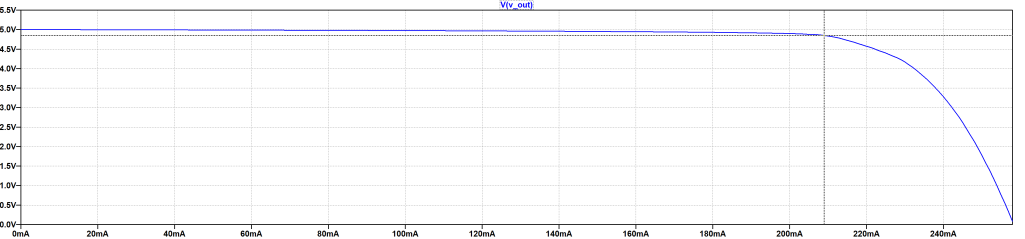
\includegraphics[width=\linewidth]{ImagenesEjercicio1/ConRpz}
	\caption{Característica de salida utilizando resistencia de polarización $R_{pz}$ = $120\Omega$}
	\label{fig:conrpz}
\end{figure}
y eso es debido a que el Zener hace mantener una respuesta constante
al permanecer polarizado. A partir de los $209 \ mA$, ya no esta dentro del rango especificado
(5 V $\pm$ 3\%). Entonces si se quita la $R_{pz}$, lo que pasará es que el diodo Zener dejará de estar polarizado al mismo tiempo que el amplificador de error entra en corte poco antes de que la protección actúe
decaiga más la tensión de salida (debido a que el Zener se empieza a despolarizar desde antes).

\begin{figure}[H]
	\centering
	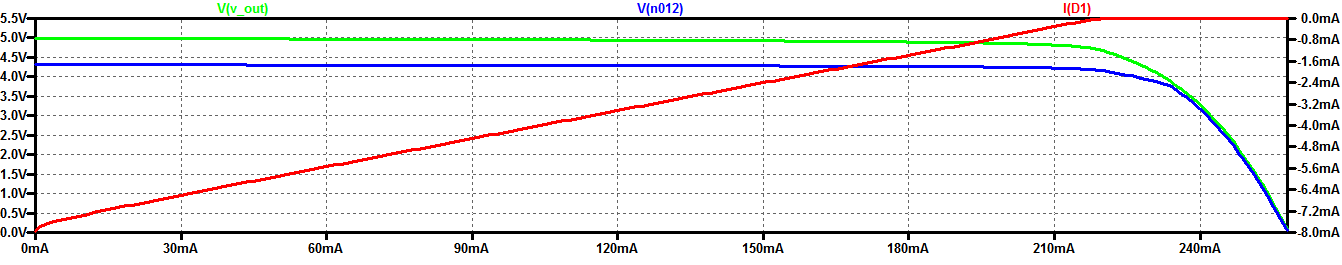
\includegraphics[width=\linewidth]{ImagenesEjercicio1/SinRpz3curvas}
	\caption{En \textcolor{green}{verde} la curva caracteristica de salida. En \textcolor{blue}{azul} la tensión sobre el diodo Zener. En \textcolor{red}{rojo} la corriente sobre el diodo Zener}
	\label{fig:sinrpz3curvas}
\end{figure}

Y así se concluye que el circuito cumple las especificaciones teniendo al diodo Zener polarizado a través
de la corriente de colector del transistor que amplifica el error.
El circuito cumple las especificaciones hasta los 202 mA

En este caso se obtiene una característica de salida similar a la anteriormente obtenida.
\begin{figure}[H]
	\centering
	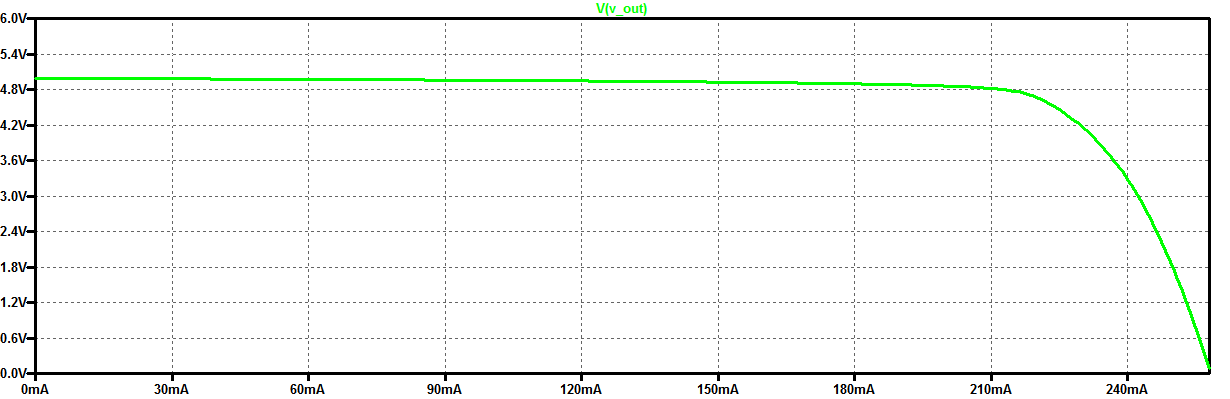
\includegraphics[width=\linewidth]{ImagenesEjercicio1/CaracteristicaDeSalidaConGrillaFL}
	\caption{}
	\label{fig:caracteristicadesalidacongrillafl}
\end{figure} 
Finalmente el circuito resultante
\begin{figure}[H]
	\centering
	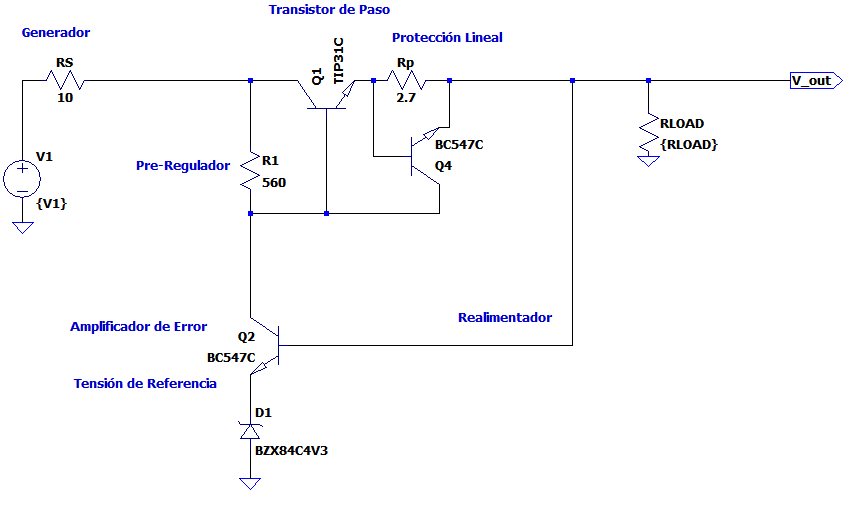
\includegraphics[width=0.7\linewidth]{ImagenesEjercicio1/ImagenCircuitoFL}
	\caption{Diseño final}
	\label{fig:imagencircuitofl}
\end{figure}



\subsubsection{Corriente constante vs Limitación de Corriente}
La incógnita restante que queda por resolver es ¿Por qué no se obtiene una respuesta abrupta a los 200 mA?
Es decir algo de esta forma:
\begin{figure}[H]
	\centering
	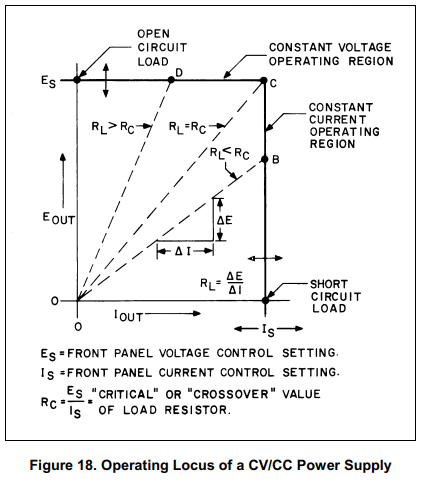
\includegraphics[scale=0.7]{ImagenesEjercicio1/CVCC}
	\caption{Característica de salida de una fuente de tensión constante con control de corriente máxima}
	\label{fig:cvcc}
\end{figure}
En la figura \ref{cvcc} se aprecia como la tensión es regulada hasta llegar a un cierto limite de corriente. A partir de ese punto, la fuente comienza a actuar como una fuente de corriente constante.

Cuando en realidad obtenemos:
\begin{figure}[H]
	\centering
	\begin{minipage}{0.45\textwidth}
		\centering
		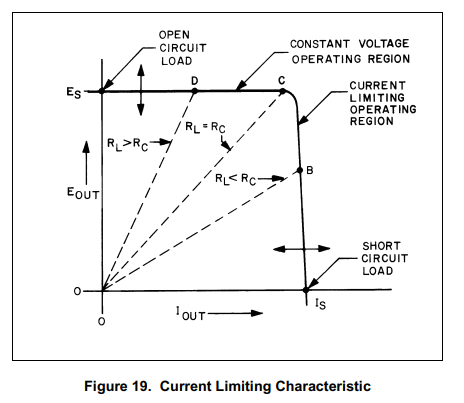
\includegraphics[width=0.9\textwidth]{ImagenesEjercicio1/CVCL.PNG} % first figure itself
		\caption{Modelo de regulador de tensión con limitador de corriente}
	\end{minipage}\hfill
	\begin{minipage}{0.45\textwidth}
		\centering
		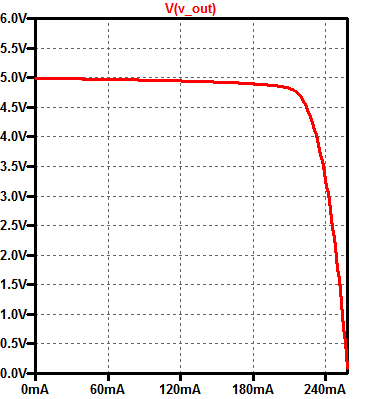
\includegraphics[width=0.9\textwidth]{ImagenesEjercicio1/CaracteristicaDeSalidaConGrillaFL2.png} % second figure itself
		\caption{Característica de Salida simulada}
	\end{minipage}
\caption*{Las imagenes fueron obtenidas \href{https://ia600205.us.archive.org/22/items/DC_Power_Supply_Handbook_Agilent_Technologies_Application_Note_90B/DC_Power_Supply_Handbook_Agilent_Technologies_Application_Note_90B.pdf}{DC Power Supply Handbook by Agilent Technologies}
}
\end{figure}

La respuesta subyace en que el circuito planteado, tanto en la etapa 1 como en la 2 del diseño, son circuitos que ofrecen limitación de la corriente máxima y no corriente constante una vez alcanzada la corriente en la que ya no se garantiza regulación de tensión. Para conseguir tal comportamiento es necesario contar con 2 circuitos  realimentados independientes. El primero de ellos sera el regulador de tensión y el segundo un regulador de corriente que deberá empezar a actuar cuando la carga utilizada exija más corriente de la permitida. En esa instancia la fuente comenzara a regular corriente. Se sabe, debido a la teoría de la realimentación negativa que para poder conseguir un buen circuito realimentado, la ganancia del amplificador debe ser varios ordenes de magnitud más grande que la ganancia del realimentador. 

\begin{figure}[H]
	\centering
	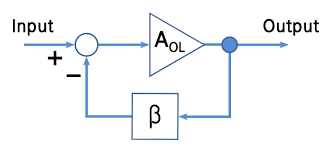
\includegraphics[scale=0.5]{ImagenesEjercicio1/Feedback}
	\caption{Diagrama en bloques de un sistema con realimentación negativa}
	\label{fig:feedback}
\end{figure}
Por lo tanto se puede concluir que en el presente diseño el lazo de realimentación que mantiene estable la corriente no tiene una gran ganancia de lazo y por ende no controla de manera muy precisa la corriente de salida.

\subsubsection{Inmunidad al ruido de linea}
Se sometió a la fuente a una prueba para verificar su estabilidad mediante a pequeños cambios en su tensión de entrada. 

\begin{figure}[H]
	\centering
	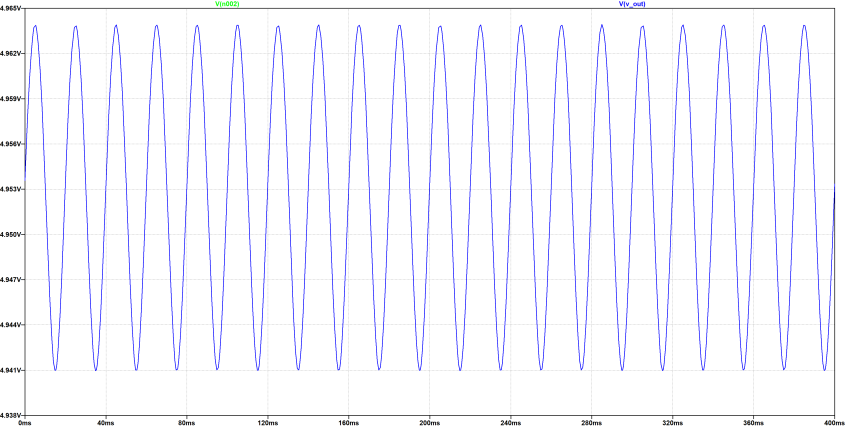
\includegraphics[width=0.7\linewidth]{ImagenesEjercicio1/InmunidadRuidoDeLinea}
	\caption{Señal de 10V DC + sinusoide de 50Hz 0.5$V_{p}$}
	\label{fig:inmunidadruidodelinea}
\end{figure}

\subsubsection{Rendimiento y potencia}
Se relevaron los datos de máxima disipación de potencia a partir de las hojas de datos de los fabricantes.


\begin{table}[H]
	\centering
	\begin{tabular}{@{}lrlll@{}}
		\toprule
		\multicolumn{1}{c}{\textbf{Componente}} & \multicolumn{1}{c}{\textbf{Maxima disipación de potencia}} &  &  &  \\ \midrule
		BC547        & 0.625W &  &  &  \\
		TIP31C       & 2W     &  &  &  \\
		BZX84C4V3    & 0.35W  &  &  &  \\ 
		Resistencias & 0.25W  &  &  &  \\ \bottomrule
	\end{tabular}
	\caption{Disipación máxima por componente}
	\label{tab:acqCap}
\end{table}


Y los rendimientos
$$\eta_{100mA} = 0.473$$

$$\eta_{200mA} = 0.487$$
\begin{equation}
H = 8 \cdot \frac{0.473 \cdot 0.487}{2\cdot 0.625W+2W+0.35W+2\cdot0.25W}
\end{equation}
\begin{equation}
	H = 44.9\%
\end{equation}